% Q9. Los chatbots me ayudan a conectar lo que aprendo en clase de matemáticas con otros conocimientos o aplicaciones prácticas
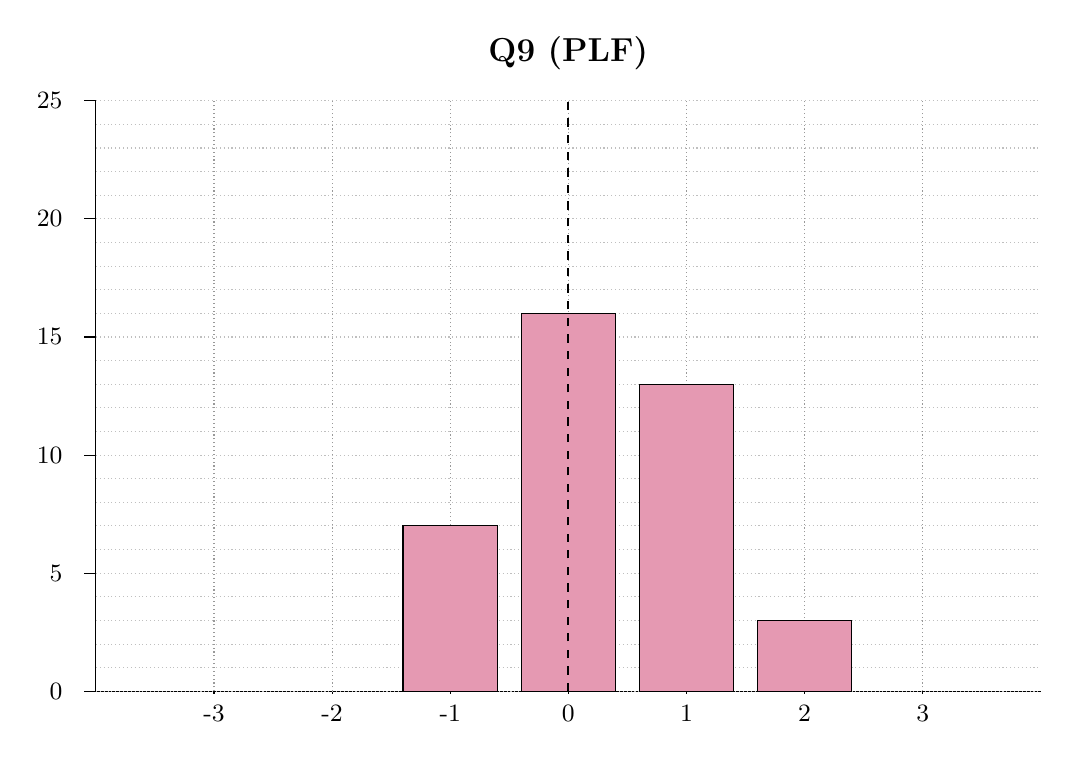
\begin{tikzpicture}[y=0.3cm, x=1.5cm]
  % Ejes
  \draw (-4,0) -- (4,0);
  \draw (-4,0) -- (-4,25); % eje y a la izquierda hasta 25

  % Cuadrícula vertical (x)
  \foreach \x in {-3,-2,-1,0,1,2,3} {
    \draw[densely dotted,gray!80] (\x,0) -- (\x,25);
    \draw (\x,-0.1) -- (\x,0);
    \node[below] at (\x,-0.2) {\small \x};
  }

  % Cuadrícula horizontal cada 1
  \foreach \y in {0,1,...,25} {
    \draw[densely dotted,gray!50] (-4,\y) -- (4,\y);
  }

  % Marcas y etiquetas cada 5 en y
  \foreach \y in {0,5,...,25} {
    \draw (-4.1,\y) -- (-4,\y);
    \node[left] at (-4.2,\y) {\small \y};
  }

  % Barras del histograma
  \fill[purple!40,draw=black] (-1.4,0) rectangle (-0.6,7);
  \fill[purple!40,draw=black] (-0.4,0) rectangle (0.4,16);
  \fill[purple!40,draw=black] (0.6,0) rectangle (1.4,13);
  \fill[purple!40,draw=black] (1.6,0) rectangle (2.4,3);

  % Línea vertical en cero (negra punteada)
  \draw[black, dashed, thick] (0,0) -- (0,25);

  % Título
  \node[font=\bfseries\large] at (0,27) {Q9 (PLF)};
\end{tikzpicture}